% **************************************************
% week_01 lecture slides
% ************************************************** 

\documentclass{beamer}

%\usepackage{mflogo}
%\usepackage{sqrcaps}
\usepackage[T1]{fontenc}

\usetheme{Rochester}
\usecolortheme{dove}
%\usefonttheme{structuresmallcapsserif}

\beamertemplatenavigationsymbolsempty

%\titlegraphic{\includegraphics[width=.25\textwidth,height=.25\textheight]{tree_math.jpg}}


\begin{document}

\title{Bayes Time \\ \vspace{0.1in} Week 01}

\author{T}
\date{2 October 2019}

%******************** 
\begin{frame}
	\vspace{-0.75in}

	\titlepage	
\end{frame}


%******************** 
\begin{frame}
	\frametitle{Outline}
	\tableofcontents
\end{frame}


% **************************************************
\section{Goals of Week 01}
% **************************************************

%******************** 
\begin{frame}
\frametitle{Goals}

\begin{enumerate}
\item
  Understand the motivation behind inference.
\item
  Appreciate the similarities and differences between Frequentist and
  Bayesian approaches to inference.
\item
  Know how to manipulate probability distributions.
\end{enumerate}

\end{frame}


\section{First things, who are we?}

%******************** 
\begin{frame}
\frametitle{Who are we?}

We are scientists who, borrowing from Karl Popper, put forward:
\begin{quote} 
Statements, or systems of statements, and test them step by step. In the field of empirical sciences, we construct hypotheses and test them against experience by observation and experiment.
\end{quote}

\bigskip

And what do we as scientists spend our time doing? As the famous physicist Richard Feynman declares 
\begin{quote} 
Experimenters search most diligently, and with the greatest effort, in exactly those places where it seems most likely that we can prove our theories wrong. In other words we are trying to prove ourselves wrong as quickly as possible, because only in that way can we find progress.
\end{quote}

\end{frame}



% **************************************************
\section{Statistical Inference}
% **************************************************

%******************** 
\begin{frame}
\frametitle{Questions}

Let's start with some questions: 
\begin{enumerate}
	\item How much will a student earn after receiving an MBA?
	\item Will the Democrats win the next US Presidential election? 
	\item Did the casino give me weighted dice to play craps? 
	\item How much do school-provided breakfasts increase student achievement?
\end{enumerate}

\end{frame}

%******************** 
\begin{frame}
\frametitle{How do we answer these questions? }

\begin{enumerate}
	\item We develop ideas about how the world works, 
	\item gather data, 
	\item construct a model, 
	\item test the model, 
	\item then see what we can say about our original query. 
\end{enumerate}

\end{frame}
	

%******************** 
\begin{frame}
\frametitle{But this is hard\ldots}

It is difficult to test those theories because we have uncertainty about how the world works (epistemological) and there are many factors outside of our control that introduce noise (ontological). Some say it is like, 
\begin{quote}
listening to a classical orchestra which is playing on the side of a busy street, while we fly overhead in a plane.
\end{quote}

\end{frame}


%******************** 
\begin{frame}
\frametitle{Luckily we have statistics}

\begin{quote}
Statistical inference is the logical framework which we can use to test our beliefs about the noisy world against data.
\end{quote}

Put slightly differently: 
\begin{quote}
Statistical inference is concerned with drawing conclusions, from numerical data, about quantities that are not observed.
Bayesian Data Analysis, 3rd edition
\end{quote}

\end{frame}

%******************** 
\begin{frame}
\frametitle{What is Bayesian inference?}

\begin{quote}
Bayesian inference is the process of fitting a probability model to a set of data and summarizing the result by a probability distribution on the parameters of the model and on unobserved quantities such as predictions for new observations.
Bayesian Data Analysis, 3rd edition
\end{quote}

\end{frame}



% **************************************************
\section{Bayesian Inference Engine}
% **************************************************

%******************** 
\begin{frame}
\frametitle{Bayesian Inference Engine}

\begin{itemize}

\item You can answer almost any question using the Bayesian inference engine that we outline below.
 
\item If you follow these steps, you will produce a set of empirically tested insights from a transparent and repeatable model that you and others can build upon. 

\item Talking to colleagues and seeking out diverse perspectives is central to your Bayesian inference efforts, and each step below presents an opportunity to consult with others.

\end{itemize}

\end{frame}

%******************** 
\begin{frame}
\frametitle{Bayesian Inference Engine}

\begin{enumerate}
\item
Develop the question
\item
Gather data, research current literature
\item
Construct model
\item
Test your code
\item
Perform prior predictive checks
\item
Estimate the model
\item
Carry out posterior predictive checks
\item
Write up your results
\end{enumerate}

\end{frame}

%******************** 
\begin{frame}
\frametitle{Way shorter way of putting it}

\begin{quote} 
We build a statistical model out of available parts and drive it as far as it can take us, and then a little farther. When the model breaks down, we dissect it and figure out what went wrong.
\end{quote}

\end{frame}

%******************** 
\begin{frame}
\frametitle{Why is this process important?}

Take it from Gelman and Shalizi in their published article \emph{Philosophy and the practice of Bayesian statistics} 
\begin{quote}
Likelihood and Bayesian inference are powerful, and with great power comes great responsibility. Complex models can and should be checked and falsified. This is how we can learn from our mistakes.
\end{quote}

\end{frame}

%******************** 
\begin{frame}
\frametitle{What do we mean by falsify?}

We know our model is wrong. It is a simplification of the complex, unwieldy world we live in. So, what do we really mean by falsify? 
\begin{quote} 
We are not interested in falsifying our model for its own sake---among other things, having built it ourselves---we know all the shortcuts taken in doing so, and can already be morally certain it is false.
\end{quote}

\end{frame}

%******************** 
\begin{frame}
\frametitle{If not falsifying, then what is the point of model checking?}

\begin{quote}
The goal of model checking, then, is not to demonstrate the foregone conclusion of falsity as such, but rather to learn how, in particular, this model fails. 
\end{quote}

Also, we would like to be able to have some faith in our results:
\begin{quote} 
If the data resembles the model closely enough, in the respects which matter to us, then reasoning based on the model will be reliable.
\end{quote}

\end{frame}

%******************** 
\begin{frame}
\frametitle{But, don't let the perfect be the enemy of the good!}

\begin{quote}
Nothing in our set of rules implies that we must run the perfect experiment (if such a thing existed) or collect all the relevant data before we can make valid social scientific inferences. An important topic is worth studying even if very little information is available.

\bigskip

The result of applying any research design in this situation will be relatively uncertain conclusions, but so long as we honestly report our uncertainty, this kind of study can be very useful. 
\end{quote}

\end{frame}

%******************** 
\begin{frame}
\frametitle{And, you know, things change}

\begin{quote}
The social world changes rapidly. To understand those changes requires that we describe them and seek to understand them contemporaneously, even when uncertainty about our conclusions is high. The urgency of a problem may be so great that data gathered by the most useful scientific methods might be obsolete before it can be accumulated. 

\bigskip

If a distraught person is running at us swinging an ax, administering a five-page questionnaire on psychopathy may not be the best strategy. 
\end{quote}

\end{frame}



% **************************************************
\section{Frequentist Inference}
% **************************************************

%******************** 
\begin{frame}
\frametitle{Frequentist World}

\begin{itemize}
	\item Frequentists suppose that the probability of flipping a coin is fixed by God.
	\item We observe noisy data that is the result of one of an infinite number of repeated experiments.
	\item Events in this infinite series of experiments occur with probabilities which represent the long-run frequencies of those events occurring in an infinite series of experimental repetitions.
 
\end{itemize}

\bigskip

\emph{Example}: We flip a coin 10 times, and it lands heads 7 times. To a frequentist this is because the universe dealt us an odd sample. See ``Rosencrantz and Guildenstern Are Dead'' by Stoppard.

\end{frame}


%******************** 
\begin{frame}
\frametitle{Frequentists summed up}

\textbf{Frequentist view the parameters of the probability model as
being fixed and the known parts of the system---the data---as varying.}

\end{frame}

% **************************************************
\section{Bayesian Worldview}
% **************************************************

%******************** 
\begin{frame}
\frametitle{Bayes' World}

\begin{itemize}
	\item Probabilities here are abstractions which we use to express our uncertainty.
	\item In a Bayesian world fictitious repetitions do not exist.
	\item In this world we witness the data and never perfectly know the value of an unknown parameter. 
\end{itemize}

\end{frame}

%******************** 
\begin{frame}
\frametitle{Philosophical aside}

\begin{itemize}
\item Is the parameter truly fixed, but our beliefs are uncertain? 
\item Or is there no definitive true probability of an event occurring, because the world is ever changing, and the system incessantly evolves? 
\end{itemize}

\end{frame}

%******************** 
\begin{frame}
\frametitle{Compare and Contrast}

\begin{itemize}
\item
  Frequentists assume data is random and originates from a series of
  infinite repetitions. Bayesians assume that we are witnesses to the
  data, which is fixed.
\item
  Frequentists view parameters as fixed features of the universe that
  represent a long-run average. Bayesian conceive of probabilities as an
  expression of subjective beliefs that can be updated in light of new
  data.
\end{itemize}

\end{frame}

%******************** 
\begin{frame}
\frametitle{Which leads to diverging paths of inference}

\begin{itemize}
\item
Frequentists use inverse probability as evidence for a given hypothesis and compute the probability of obtaining a sample as extreme as or more than the one actually obtained assuming a hypothesis is true.
\item
Bayes' formula circumvents the problem of generating fictious samples by inverting the Frequentist probability to obtain the probability of the hypothesis given the data we obtained.
\end{itemize}

\end{frame}


% **************************************************
\section{Introduction to Probability Distributions}
% **************************************************


%******************** 
\begin{frame}
\frametitle{Probability Distributions are central to Bayesian inference}

In Bayesian models we quantify uncertainty with probability distributions. 

\bigskip

We input probability distributions to Bayes' rule and the output we receive is a probability distribution, so we need to be comfortable with these objects.

\end{frame}


%******************** 
\begin{frame}
\frametitle{Random variables}

\textbf{Definition} Given an experiment with sample space, $S$, a \emph{random variable} is a function from the sample space $S$ to the real numbers $\mathbb{R}$.

\bigskip

A random variable $X$ assigns a numerical value $X(s)$ to each possible outcome of the experiment. Randomness stems from the fact that the outcome of our experiment is random and described by our probability function $P$.

\end{frame}


%******************** 
\begin{frame}
\frametitle{Example random variable}

\textbf{Example}: Suppose we toss a fair coin twice. The sample space $S = \{HH, HT, TH, TT\}$. Let $X$ be the number of heads. This is a random variable with possible values 0, 1, and 2. 

\bigskip

$X$ assigns values to each outcome: 
\begin{itemize}
\item X(HH) = 2 
\item X(HT) = 1 
\item X(TH) = 1 
\item X(TT) = 0
\end{itemize}

\end{frame}


%******************** 
\begin{frame}
\frametitle{Discrete Probability Distributions}

\textbf{Definition} Given an experiment with sample space, $S$, a random variable is a \emph{discrete random variable} if there is a finite list of values $a_1, a_2, \ldots, a_n$ or an infinite list of values $a_1, a_2, \ldots$ such that $P(X = a_j \,\textrm{for some} \, j) = 1$. 

\bigskip

The set of values $x$ such that $P(X = x) > 0$ is called the support of $X$.

\end{frame}


%******************** 
\begin{frame}
\frametitle{Probability Mass Function}

\textbf{Definition} The \emph{probability mass function} of a discrete random variable $X$ is the function $p_X$ given by $p_X(x) = P(X = x)$. This function is positive if $x$ is in the support of $X$,  and $0$ otherwise. 

\bigskip 

\begin{enumerate}
\item 
PMFs are non-negative, $p_X(x) > 0$ if  $x = x_j$ for some $j$, and $p_X(x) = 0$ otherwise. 
\item
PMFs sum to 1: $\sum_{j=1}^{\infty} p_X(x_j) = 1$.
\end{enumerate}

\bigskip

Note, $X = x$ is an event consisting of all outcomes $s$ to which $X$ assigns the number $x$. Formally, we write this as $\{s \in S : X(s) = x\}$.

\end{frame}

%******************** 
\begin{frame}
\frametitle{Example}

Suppose we flip a fair coin twice. What is the PMF? 

\bigskip

\begin{itemize}
	\item $p_X(0) = P(X = 0) = \frac{1}{4}$ 
	\item $p_X(1) = P(X = 1) = \frac{1}{2}$ 
	\item $p_X(2) = P(X = 2) = \frac{1}{4}$ 
\end{itemize}

\end{frame}



%******************** 
\begin{frame}
\frametitle{Another example}

\textbf{Example}: (if time) We roll two fair 6-sided dice. Let $T = X + Y$ be the total of the two rolls, where $X$ and $Y$ are the individual rolls. The sample space has 36 equally likely outcomes: $S = \{(1,1), (1,2), \ldots,(6,6)\}$

\bigskip

What is the PMF of T? 
\begin{itemize}
	\item $P(T=2) = P(T=12) = \frac{1}{36}$ 
	\item $P(T=3) = P(T=11) = \frac{2}{36}$
	\item $P(T=4) = P(T=10) = \frac{3}{36}$ 
	\item $P(T=5) = P(T=9) = \frac{4}{36}$ 
	\item $P(T=6) = P(T=8) = \frac{5}{36}$
	\item $P(T=7) = \frac{6}{36}$
\end{itemize}

\end{frame}


%******************** 
\begin{frame}
\frametitle{Our first probability distribution}

\textbf{Definition} A random variable $X$ has the Bernoulli distribution with parameter $p$, if $P(X = 1) = p$ and $P(X = 0) = 1 - p$, where $0 < p < 1$. We write this as $X \sim \text{Bernouli}(p)$. ($\sim$ is read as ``distributed as'')

\bigskip

Any event has a Bernoulli random variable associated with it, equal to 1 if the event happens and 0 otherwise. If the event is a ``success'' or a ``failure'' we can call it a Bernoulli trial.

\end{frame}

%******************** 
\begin{frame}
\frametitle{Aa quick detour to count things\ldots}

\textbf{Definition} For any nonnegative integers $n$ and $k$, the binomial coefficient $\binom{n}{k}$, said ``n choose k'', is the number of subsets of size $k$ for a set of size $n$ and equals 
\begin{equation}
	\frac{n!}{(n - k)! * k!}
\end{equation}

\end{frame}


%******************** 
\begin{frame}
\frametitle{Expanding our world a bit}

Suppose that we have a series of $N$ Bernoulli trials, how is that distributed? 

\end{frame}

%******************** 
\begin{frame}
\frametitle{Your second probability distribution}

\textbf{Defintion} Suppose that n independent Bernoulli trials are performed, each with the same success probability $p$. Let $X$ be the number of successes. 

\bigskip

The distribution of $X$ is called the binomial distribution with parameters $n$ and $p$. We write $X \sim \text{Binomial}(n,p)$, where $n$ is a positive integer and $0 < p < 1$.

\end{frame}


%******************** 
\begin{frame}
\frametitle{Binomial Probability Mass Function}

\textbf{Definition} (Binomial PMF) If $X \sim \text{Binomial}(n,p)$, then the PMF of $X$ is 
\begin{equation}
P(X = k) = \binom{n}{k} p^{k} (1-p)^{(n-k)}
\end{equation}
for k = 0, 1, \ldots, n; and $P(X = k) = 0$ otherwise.

\end{frame}


%******************** 
\begin{frame}
\frametitle{Example binomial PMFs}

\begin{center}
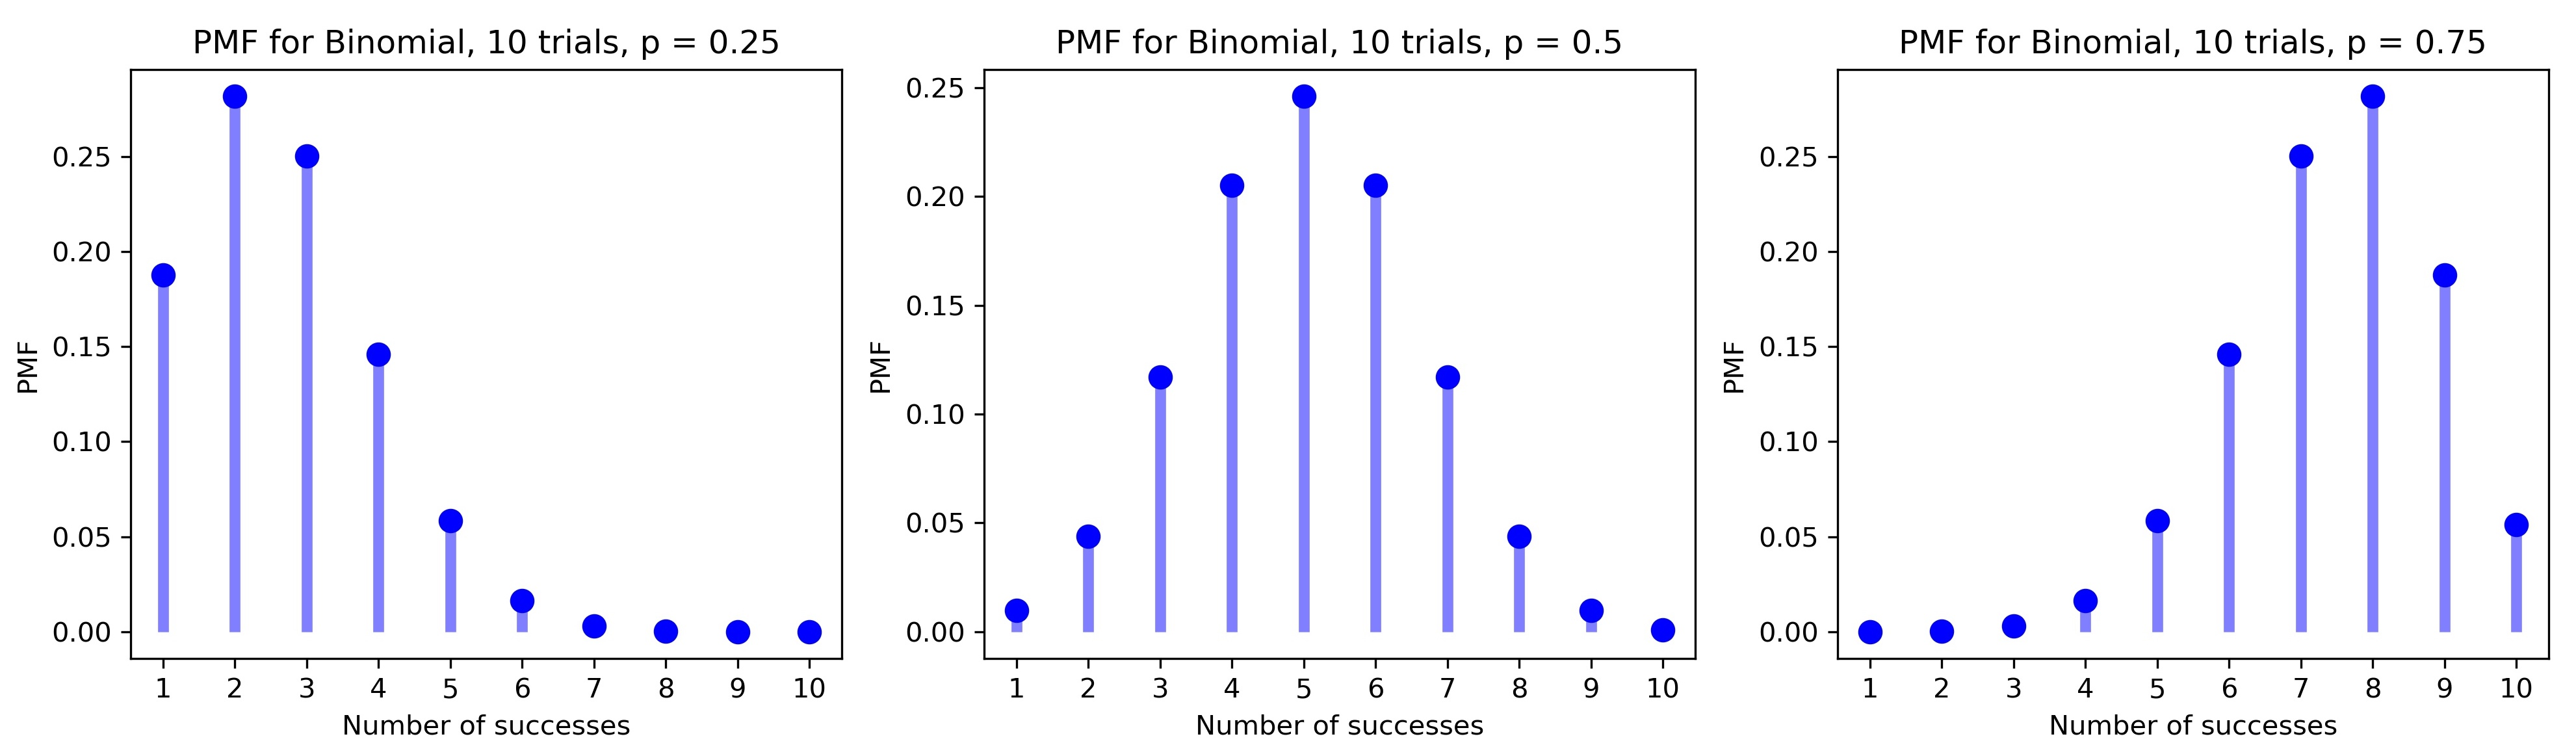
\includegraphics[width=4.35in]{binomial_pmfs.jpg}
\end{center}

\end{frame}



%******************** 
\begin{frame}
\frametitle{Cumulative Distribution Function}

\textbf{Definition} The cumulative distribution function of a random variable $X$ is the function $F_X$ given by $F_X(x) = P(X \leq x)$.

\bigskip
\begin{enumerate}
\item
The CDF is increasing in x, if $x_1 \leq x_2$ then $F_X(x_1) \leq F(x_2)$. 

\bigskip

\item
The CDF converges to 0 in the limit as $x$ approaches $-\infty$; and converges to 1 in the limit as $x$ approaches $\infty$.
\end{enumerate}


\end{frame}


%******************** 
\begin{frame}
\frametitle{Example Binomial PMF and CDF}

\begin{center}
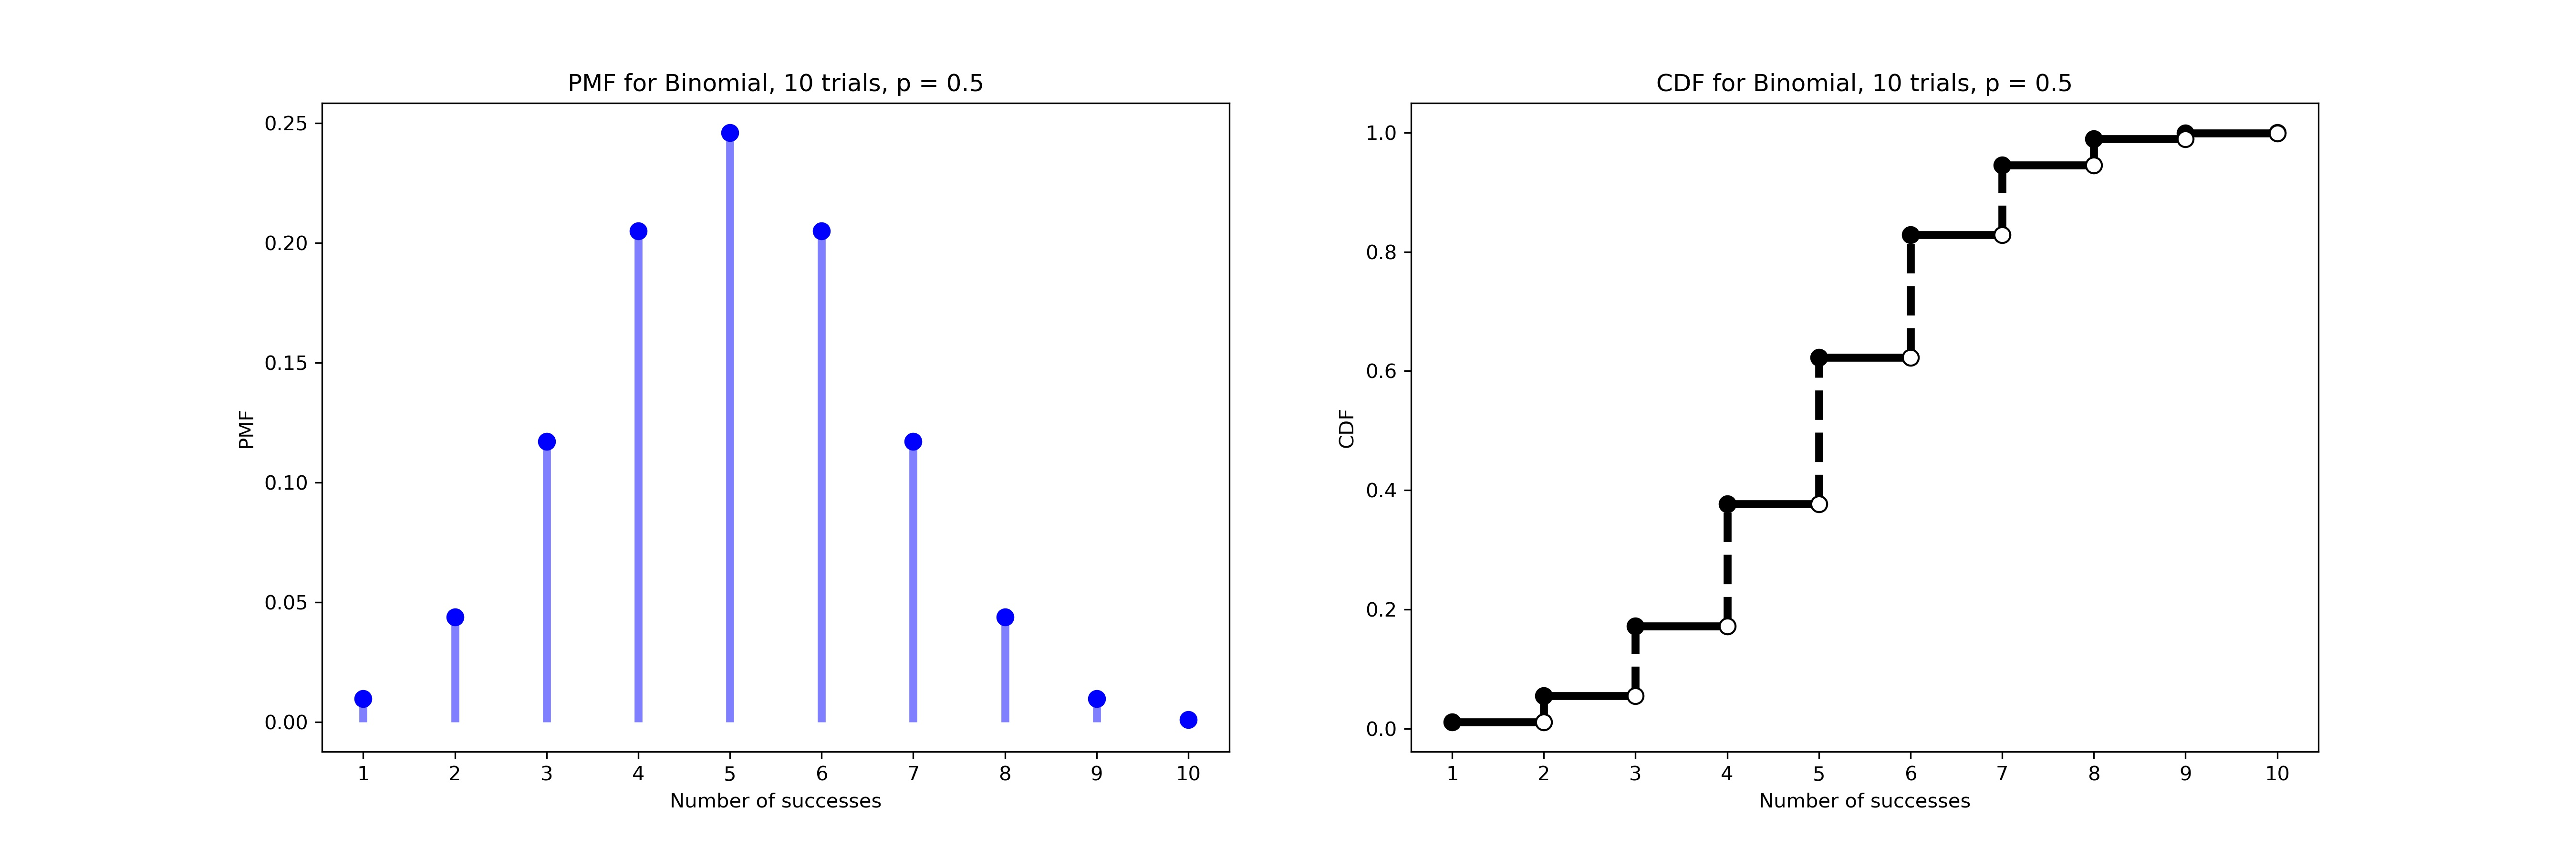
\includegraphics[width=4.75in]{binomial_pmf_cdf.jpg}
\end{center}

\end{frame}



%******************** 
\begin{frame}
\frametitle{Continuous random variables}

Continuous random variables can take on any real value in an interval. For example: the wing span of an eagle, the height of a person, the length of time until a light bulb burns out.

\bigskip

\textbf{Definition} A random variable has a continuous distribution if the CDF is differentiable.

\end{frame}


%******************** 
\begin{frame}
\frametitle{Cumulative Distribution Function, Continuous Version}

\textbf{Definition} For a continuous random variable $X$ with CDF $F$, the probability density function of $X$ is the derivative of the CDF, given by $f_X(x) = F'(x)$. The support of $X$, and of its distribution, is the set of all $x$ where $f(x) > 0$. Valid PDFs are nonnegative, $f(x) \geq 0$; and integrate to 1, $\int_{-\infty}^{+\infty} f(x)dx = 1$.

\bigskip

A key difference between discrete and continuous random variables is that for a continuous random variable, the PMF, $P(X=x) = 0$ for all $x$. $P(X = x)$ is the height of a jump in the CDF at $x$, but the CDF of $X$ has no jumps!


\end{frame}



%******************** 
\begin{frame}
\frametitle{The Uniform Distribution}

\textbf{Definition} A continuous random variable $U$ is said to have the uniform distribution on the interval $(a,b)$ if its PDF is

\bigskip

\begin{equation}
f(x) = 
	\begin{cases} 
		\frac{1}{b-a} & a < x < b \\
		0 & \textrm{otherwise} 
   \end{cases}
\end{equation}

\end{frame}



%******************** 
\begin{frame}
\frametitle{Normal (Gaussian) Distribution}

The normal distribution is the ``bell-shaped curve'' everyone always talks about. It is widely used in statistics, because of the Central Limit Theorem which says that under weak assumptions, the sum of a large number of independent and identically distributed random variables has an approximately normal distribution.

\end{frame}


%******************** 
\begin{frame}
\frametitle{Standard Normal PDF}

\textbf{Definition} A continuous random variable $Z$ is said to have the standard Normal distribution if its PDF is given by:

\bigskip

\begin{equation}
	f(z) = \frac{1}{\sqrt{2 \pi}} \exp \left(\frac{-z^{2}}{2} \right), \textrm{for} -\infty < z < \infty
\end{equation}

\bigskip

$\frac{1}{\sqrt{2\pi}}$ is a normalizing constant that makes the PDF sum to $1$.

\end{frame}


%******************** 
\begin{frame}
\frametitle{Why is the normal distribution so common?}

Suppose you and a thousand of your closest friends line up on the halfway line of a soccer field. Each of you has a coin in your hand. At the sound of a whistle, you begin flipping the coins. Each time a coin comes up heads, that person moves one step towards the left-hand goal. Each time a coin comes up tails, that person moves one step towards the right-hand goal.

\bigskip

Each person flips the coin 16 times, follows the implied moves, and then stands still. Now we measure the distance of each person from the halfway line. Can you predict the proportion of people who are standing on the halfway line? How about the proportion 5 yards away? We claim that the distribution of people around the halfway line will be approximately normal.

\end{frame}


%******************** 
\begin{frame}
\frametitle{Did you imagine something like this?}

\begin{center}
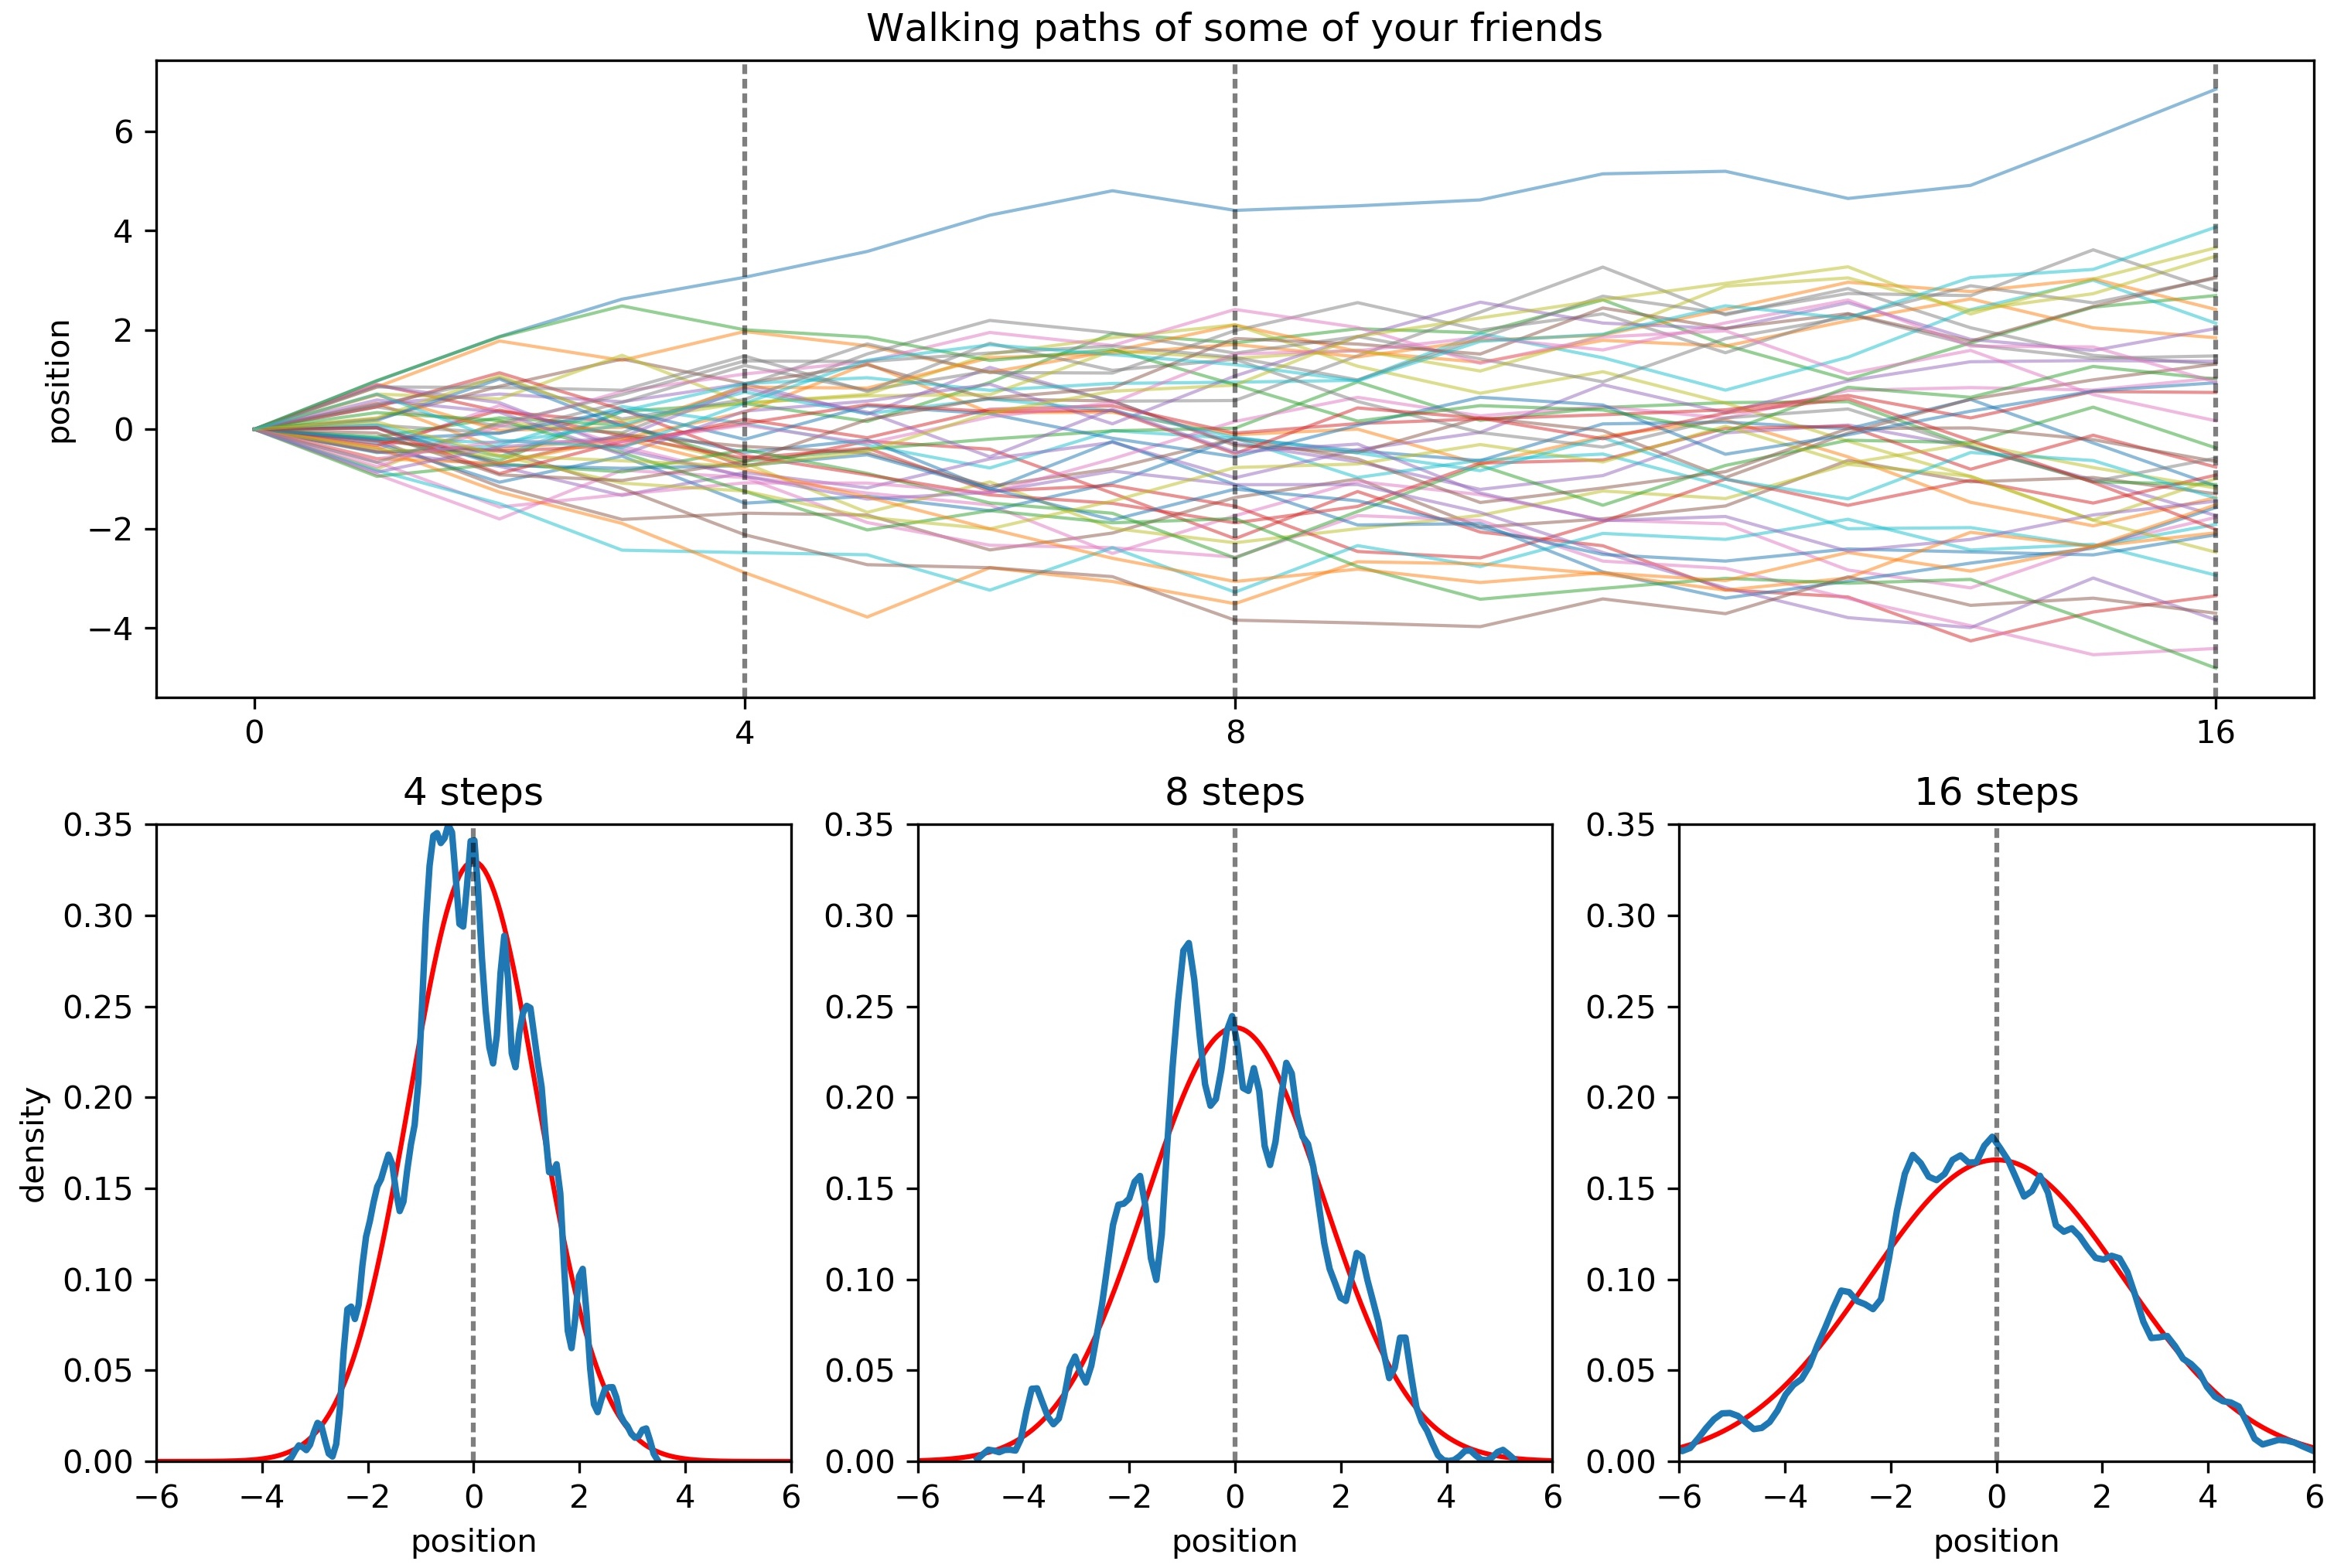
\includegraphics[width=4in]{random_walkers.jpg}
\end{center}

\end{frame}


%******************** 
\begin{frame}
\frametitle{Why might we use the Normal distribution as a base case?}

\textbf{Ontological justification}

\bigskip

The world is full of Gaussian distributions, approximately. It is a widespread pattern appearing in measurement errors, variations in growth, and the velocities of molecules. At their heart these processes add together fluctuations, and repeatedly adding fluctuations results in a distribution of sums that have shed all information about the underlying process except for the mean and spread.

\end{frame}



%******************** 
\begin{frame}
\frametitle{Why might we use the Normal distribution as a base case?}

\textbf{Epistemological Justification}

\bigskip

If all we are willing to say about the distribution of a measure is the mean and variance, then the Gaussian distribution is most consistent with our assumptions. If we assume the measure has finite variance, then the Gaussian distribution is the shape that can be realized in the largest number of ways and does not introduce any new assumptions, ie it is the least surprising and least informative assumption we can make.

\end{frame}

% **************************************************
\section{Application of Bayes rule}
% **************************************************

%******************** 
\begin{frame}
\frametitle{Example: estimating a rate from Poisson data}

\begin{itemize}
	\item In one US county, It is found that 3 people out of a population of 200,000 died of asthma in a single year.
	
	\item A Poisson sampling model is often used for data of this form.
	
	\item The Poisson distribution is a discrete probability distribution that expresses the probability of a given number of events occurring in a fixed interval of time or space if these events occur with a known constant rate ($\lambda > 0$) and independently of the time since the last event.

	\item How can we build a Bayesian model to help us estimate the actual rate of disease?
\end{itemize}


\end{frame}

%******************** 
\begin{frame}
\frametitle{Example of a Poisson PMF and CDF}

\begin{center}
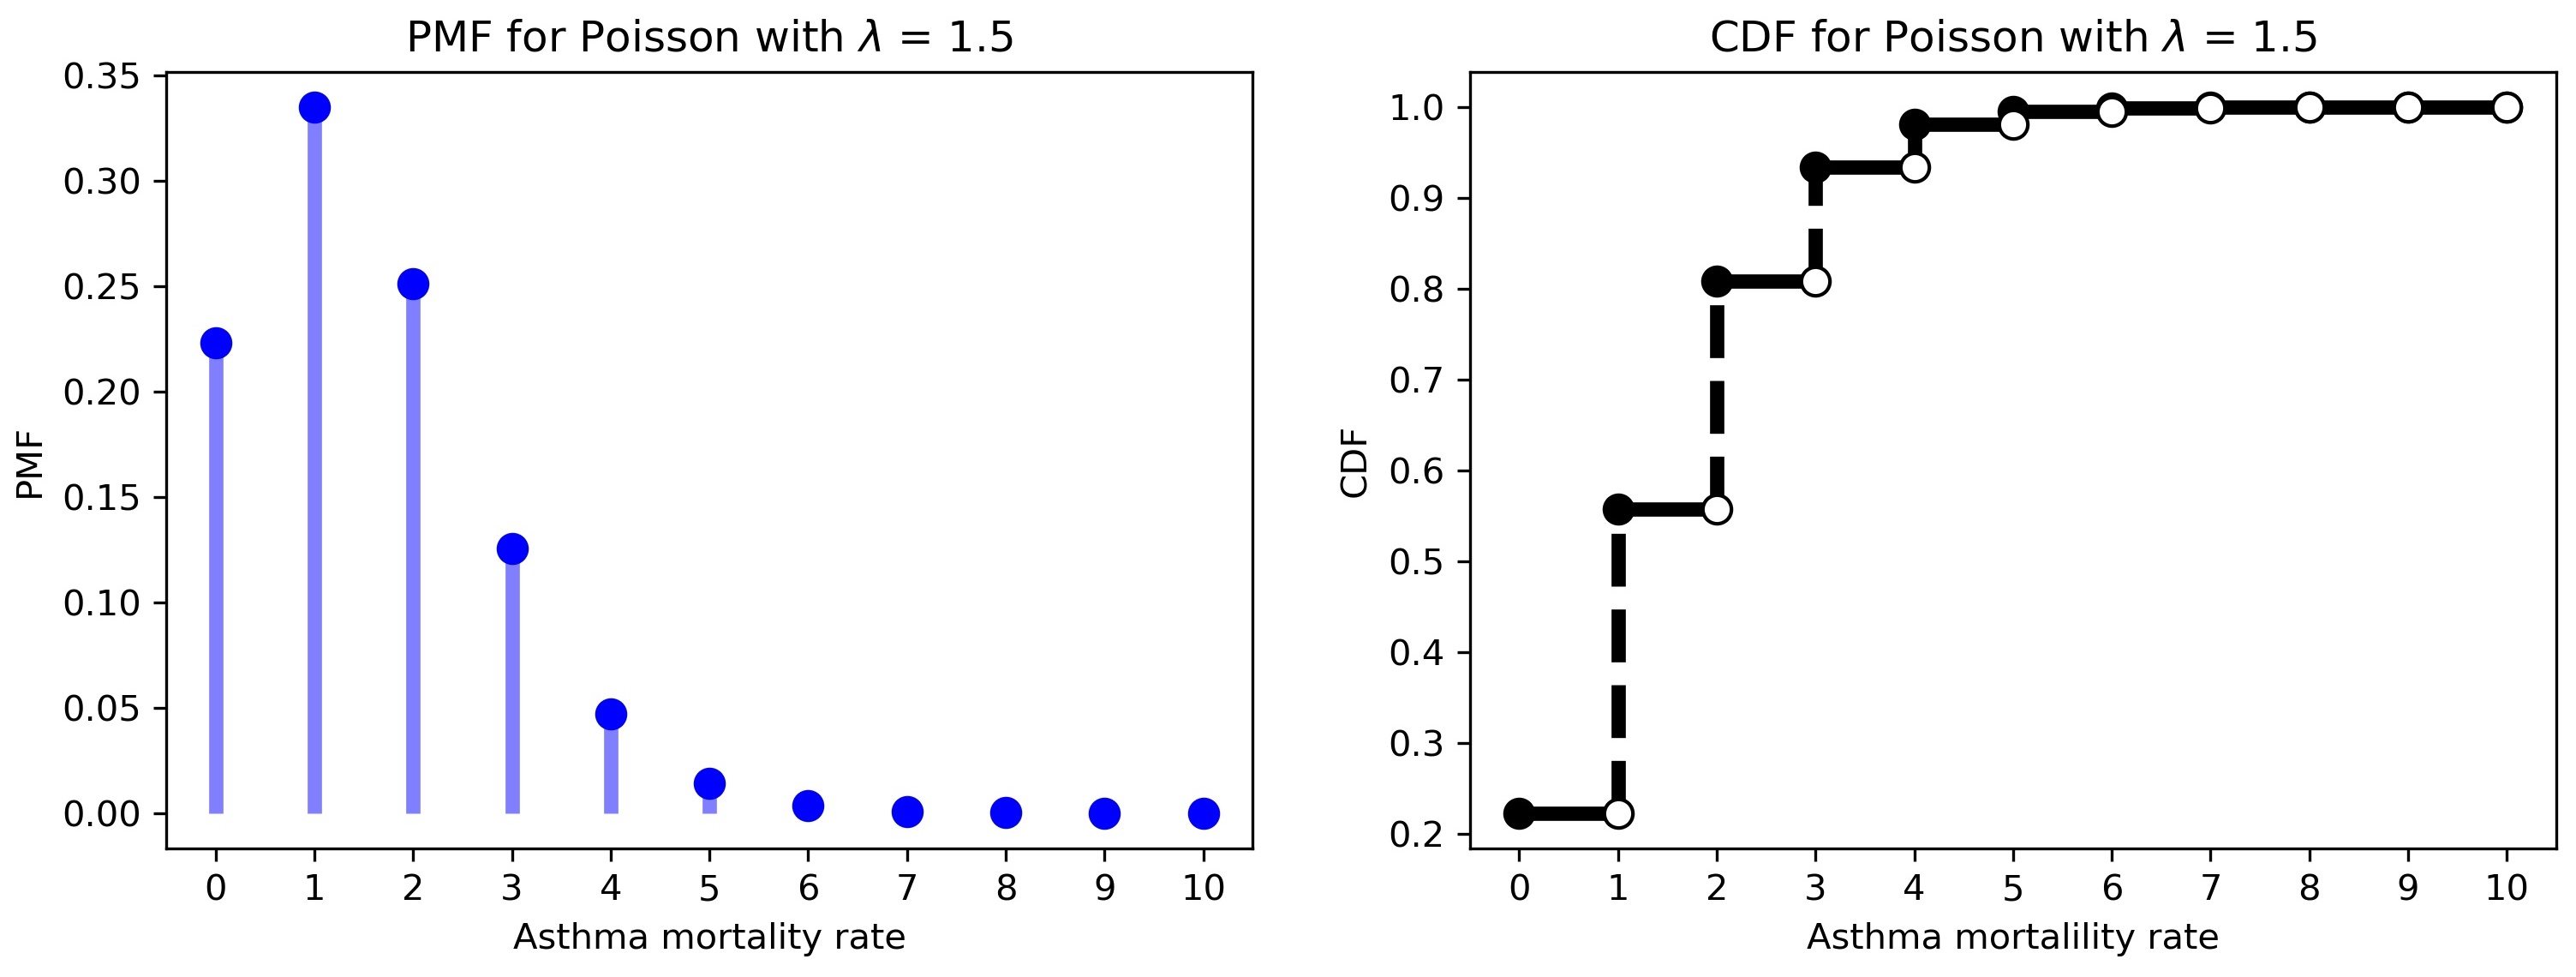
\includegraphics[width=4in]{poisson_pfm_cdf.jpg}
\end{center}

\end{frame}


%******************** 
\begin{frame}
\frametitle{Bayes' Rule}

\begin{equation}
	P(\lambda | x = 1.5) = \frac{P(x=1.5| \lambda) P(\lambda)}{P(x=1.5)}
\end{equation}

\end{frame}

%******************** 
\begin{frame}
\frametitle{What is $P(\lambda)$?}

\begin{itemize}
	\item $P(\lambda)$ is our prior distribution for the rate of asthma mortality rate.
	
	\item We know that a Poisson rate must be greater than zero. So what kind of probability distribution can we place on $\lambda$ to reflect our prior knowledge?
	
	\item Suppose we know that mortality rates in countries similar to the US are rarely above 1.5 per 100,000 people, with typical rates around 0.6. 

\end{itemize}

\end{frame}


%******************** 
\begin{frame}
\frametitle{A reasonable prior}

We pick a prior of Gamma(3.0,5.0), because it matches our prior knowledge, and its support is greater than zero.

\begin{center}
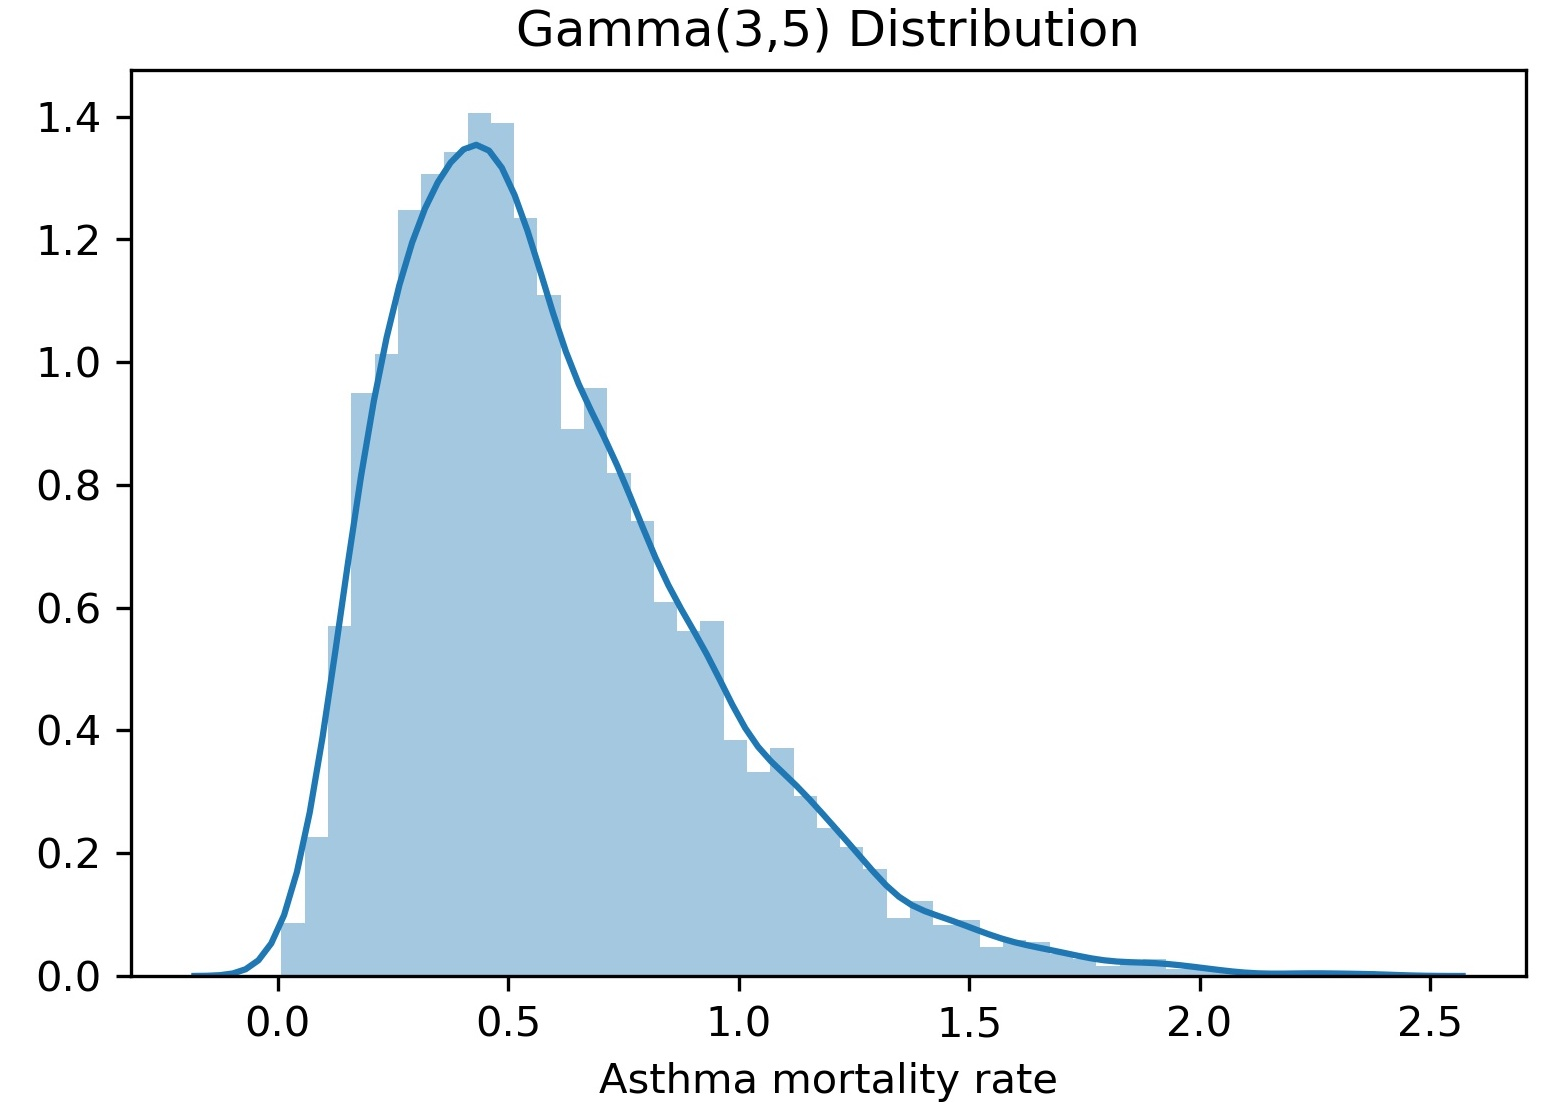
\includegraphics[width=3in]{gamma_3_5_pdf.jpg}
\end{center}


\end{frame}

%******************** 
\begin{frame}
\frametitle{What's next?}

\begin{itemize}
	\item We specificed our prior, Gamma(3,5).
	\item We also specified our likelihood, $\textrm{Poisson}(x=1.5 | \lambda)$.
	\item Now we can run our black box inference machine to compute our posterior density.
	\item We will learn how this inference machine works next week, but, for now, trust us that the posterior distribution looks like this\ldots
\end{itemize}

\end{frame}


%******************** 
\begin{frame}
\frametitle{Posterior on asthma mortality rates}

\begin{center}
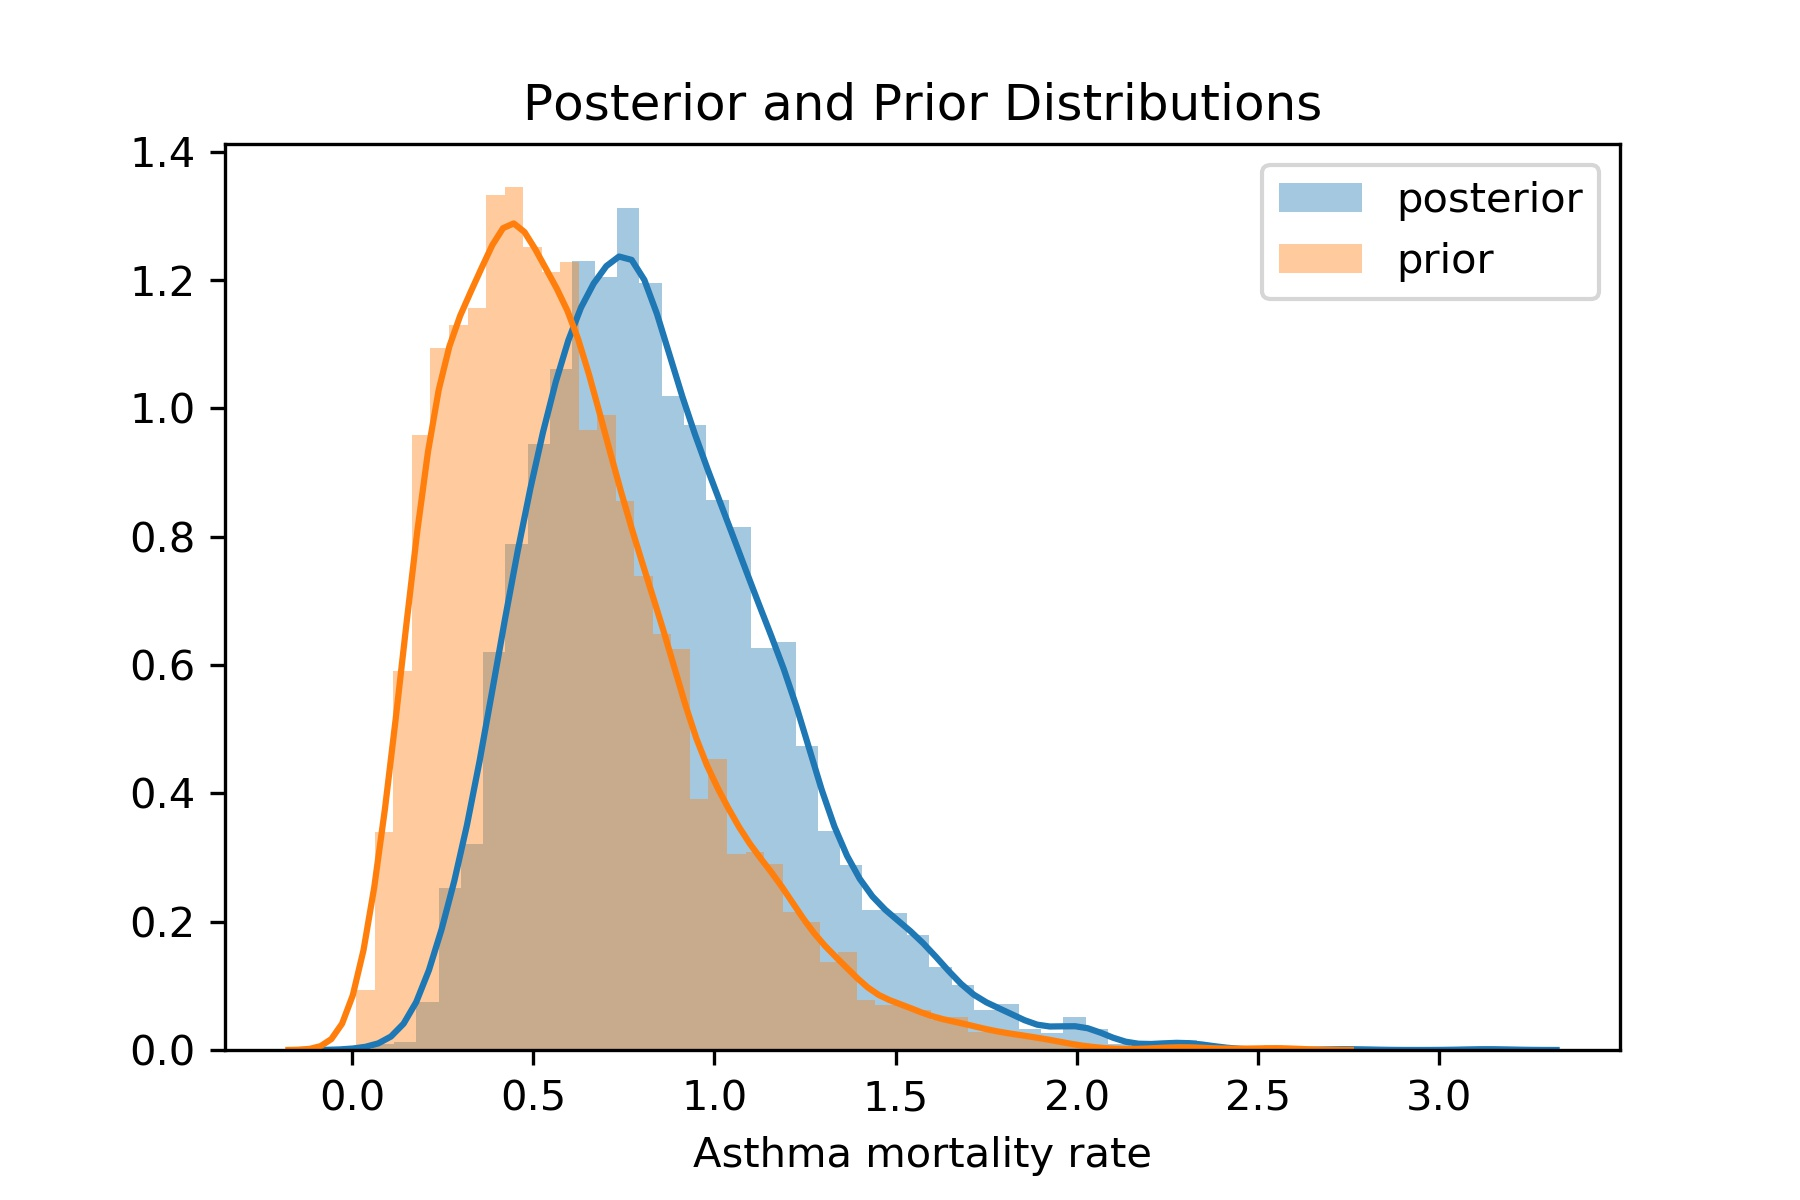
\includegraphics[width=3in]{asthma_posterior.jpg}
\end{center}


\end{frame}



\end{document} 
